% =============================================================================
% Module 9.0: Security Concepts
% Network+ Course - LaTeX Beamer Presentation
% Theme: The Adventures of Agent Snoopy
% =============================================================================

\documentclass[aspectratio=169, 11pt]{beamer}

% Theme and colors
\usetheme{Madrid}
\usecolortheme{default}

% Custom colors
\definecolor{rctcblue}{RGB}{0, 74, 136}
\definecolor{rctcgold}{RGB}{255, 199, 44}
\definecolor{networkgreen}{RGB}{0, 150, 100}
\definecolor{alertred}{RGB}{200, 50, 50}
\definecolor{aborange}{RGB}{230, 120, 0}
\definecolor{tcpblue}{RGB}{30, 100, 180}
\definecolor{udpgreen}{RGB}{50, 160, 80}

% Set theme colors
\setbeamercolor{palette primary}{bg=rctcblue, fg=white}
\setbeamercolor{palette secondary}{bg=rctcblue!80, fg=white}
\setbeamercolor{palette tertiary}{bg=rctcblue!60, fg=white}
\setbeamercolor{structure}{fg=rctcblue}
\setbeamercolor{title}{fg=rctcblue}
\setbeamercolor{frametitle}{fg=rctcblue, bg=rctcblue!10}
\setbeamercolor{block title}{bg=rctcblue, fg=white}
\setbeamercolor{block body}{bg=rctcblue!5}
\setbeamercolor{block title alerted}{bg=alertred, fg=white}
\setbeamercolor{block body alerted}{bg=alertred!5}
\setbeamercolor{block title example}{bg=networkgreen, fg=white}
\setbeamercolor{block body example}{bg=networkgreen!5}

% Packages
\usepackage{tikz}
\usepackage{booktabs}
\usepackage{fontawesome5}
\usepackage{graphicx}
\usepackage{xcolor}
\usepackage{colortbl}
\usepackage{array}
\usepackage{listings}
\usepackage{amsmath}
\usepackage{amssymb}

% TikZ libraries (Including the fix for snake decoration)
\usetikzlibrary{shapes.geometric, arrows.meta, positioning, decorations.pathreplacing, 
                backgrounds, fit, calc, shadows, shapes.symbols, shapes.misc, decorations.pathmorphing}

% TikZ Styles
\tikzstyle{process} = [draw=rctcblue, fill=rctcblue!15, rounded corners,
                       minimum width=1.8cm, minimum height=0.5cm, font=\footnotesize, align=center]
\tikzstyle{attacker} = [draw=alertred, fill=alertred!15, rounded corners, font=\footnotesize]

% Icon commands (Using custom PNG icons from images/icons/ where available)
\newcommand{\iconpc}[1][0.6cm]{\resizebox{#1}{!}{
\includegraphics{images/icons/icon_pc.png}}}
\newcommand{\iconserver}[1][0.6cm]{\resizebox{#1}{!}{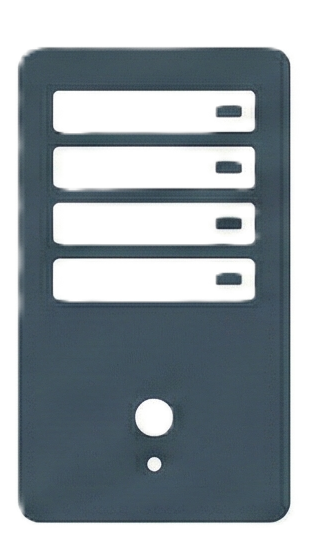
\includegraphics{images/icons/icon_server.png}}}
\newcommand{\iconrouter}[1][0.6cm]{\resizebox{#1}{!}{
\includegraphics{images/icons/icon_router.png}}}
\newcommand{\iconswitch}[1][0.6cm]{\resizebox{#1}{!}{
\includegraphics{images/icons/icon_switch.png}}}
\newcommand{\iconfirewall}[1][0.6cm]{\resizebox{#1}{!}{
\includegraphics{images/icons/icon_firewall.png}}}
\newcommand{\iconcloud}[1][0.6cm]{\resizebox{#1}{!}{
\includegraphics{images/icons/icon_cloud.png}}}
\newcommand{\iconlock}[1][0.6cm]{\resizebox{#1}{!}{
\includegraphics{images/icons/icon_lock.png}}}
\newcommand{\iconuser}[1][0.6cm]{\resizebox{#1}{!}{\faIcon{user}}}
\newcommand{\iconhacker}[1][0.6cm]{\resizebox{#1}{!}{\faIcon{user-secret}}}
\newcommand{\iconkey}[1][0.6cm]{\resizebox{#1}{!}{\faIcon{key}}}
\newcommand{\iconfile}[1][0.6cm]{\resizebox{#1}{!}{\faIcon{file-alt}}}
\newcommand{\icondatabase}[1][0.6cm]{\resizebox{#1}{!}{
\includegraphics{images/icons/icon_db.png}}}
\newcommand{\icondog}[1][0.6cm]{\resizebox{#1}{!}{\faIcon{dog}}}
\newcommand{\iconcat}[1][0.6cm]{\resizebox{#1}{!}{\faIcon{cat}}}

% Document info
\title[Security Concepts]{Module 9.0: Security Concepts}
\subtitle{Intro to Networks}
\author{Brendan Shea, PhD}
\institute{Rochester Community and Technical College}
\date{}

\begin{document}

% =============================================================================
% Module 9.0: Security Concepts (Slides 1-10 Enhanced)
% =============================================================================

% SLIDE 1: Title (Fixed Alignment)
\begin{frame}
    \titlepage
    \begin{center}
        
\begin{tikzpicture}[scale=0.8]
            % Shield
            \node[font=\Huge, text=rctcblue] (shield) at (0, 0) {\faIcon{shield-alt}};
            
            % Agent Snoopy (The Defender)
            \node (snoopy) at (-2.5, 0) {\icondog[1.2cm]};
            \node[below=0.1cm of snoopy, font=\bfseries\tiny, text=rctcblue, align=center] {Agent Snoopy\\(KibbleCorp Security)};
            
            % The Threat (Hacker Cat)
            \node (cat) at (2.5, 0) {\iconcat[1.2cm]};
            \node[below=0.1cm of cat, font=\bfseries\tiny, text=alertred, align=center] {The Hacker Cat\\(Threat Actor)};
            
            % Arrows
            \draw[->, ultra thick, networkgreen] (snoopy) -- (shield);
            \draw[->, ultra thick, alertred, dashed] (cat) -- (shield);
        \end{tikzpicture}
    \end{center}
\end{frame}

% SLIDE 2: Roadmap
\begin{frame}{Module 9 Roadmap}
    \begin{center}
        \begin{tikzpicture}[scale=0.85, transform shape]
            \node[process] (concepts) at (0, 3) {9.1 Concepts};
            \node[process] (threats) at (3, 1.5) {9.2 Threats};
            \node[process] (spoofing) at (6, 3) {9.3 Spoofing};
            \node[process] (rogue) at (9, 1.5) {9.4 Rogue Systems};
            \node[process] (social) at (12, 3) {9.5 Social Eng.};

            \draw[->, thick, rctcblue] (concepts) -- (threats);
            \draw[->, thick, rctcblue] (threats) -- (spoofing);
            \draw[->, thick, rctcblue] (spoofing) -- (rogue);
            \draw[->, thick, rctcblue] (rogue) -- (social);

            \node[below=0.1cm of concepts] {\iconlock[0.5cm]};
            \node[below=0.1cm of threats] {\iconhacker[0.5cm]};
            \node[below=0.1cm of spoofing] {\faIcon{mask}};
            \node[below=0.1cm of rogue] {\faIcon{wifi}};
            \node[below=0.1cm of social] {\faIcon{user-tie}};
        \end{tikzpicture}
    \end{center}
    \vspace{0.5cm}
    \begin{alertblock}{The Mission}
        \footnotesize
        Help Agent Snoopy defend the KibbleCorp network from the Hacker Cat's attacks using industry-standard tools and techniques.
    \end{alertblock}
\end{frame}

% SLIDE 3: CIA Triad (Analogy Enhanced)
\begin{frame}{9.1 Security Terminology: The CIA Triad}
    \begin{columns}[T]
        \begin{column}{0.5\textwidth}
            \begin{block}{The Holy Trinity of Security}
                \footnotesize
                \begin{itemize}\setlength{\itemsep}{2pt}
                    \item \textbf{Confidentiality} (Secrecy)
                    \begin{itemize}\setlength{\itemsep}{0pt}
                        \item Only authorized people can see data.
                        \item \textit{Analogy:} A diary with a lock.
                    \end{itemize}
                    \item \textbf{Integrity} (Accuracy)
                    \begin{itemize}\setlength{\itemsep}{0pt}
                        \item Data hasn't been changed or tampered with.
                        \item \textit{Analogy:} A sealed food jar (safety seal).
                    \end{itemize}
                    \item \textbf{Availability} (Uptime)
                    \begin{itemize}\setlength{\itemsep}{0pt}
                        \item Data is accessible when needed.
                        \item \textit{Analogy:} A 24/7 convenience store.
                    \end{itemize}
                \end{itemize}
            \end{block}
        \end{column}
        \begin{column}{0.48\textwidth}
            \begin{center}
                \begin{tikzpicture}[scale=0.7]
                    \node (c) at (0, 3) {\iconlock[0.8cm]};
                    \node[above] at (0, 3.4) {\textbf{Confidentiality}};
                    \node (i) at (-2.5, -1) {\iconfile[0.8cm]};
                    \node[below] at (-2.5, -1.4) {\textbf{Integrity}};
                    \node (a) at (2.5, -1) {\faIcon{clock}};
                    \node[below] at (2.5, -1.4) {\textbf{Availability}};
                    \draw[ultra thick, rctcblue] (c) -- (i);
                    \draw[ultra thick, rctcblue] (i) -- (a);
                    \draw[ultra thick, rctcblue] (a) -- (c);
                    \node[font=\bfseries\Large, text=rctcgold] at (0, 0.5) {CIA};
                \end{tikzpicture}
            \end{center}
        \end{column}
    \end{columns}
\end{frame}

% SLIDE 4: Audits & Compliance (Detail Enhanced)
\begin{frame}{Audits \& Compliance}
    \begin{columns}[T]
        \begin{column}{0.48\textwidth}
            \begin{block}{Security Audits}
                \footnotesize
                Why audit? To find broken locks before thieves do.
                \begin{itemize}
                    \item \textbf{Internal}: Snoopy checking his own doors.
                    \item \textbf{External}: Hiring a pro to break in (Pen Test).
                \end{itemize}
            \end{block}
            \begin{alertblock}{Regulatory Compliance (The Law)}
                \footnotesize
                \begin{itemize}
                    \item \textbf{HIPAA} (Health): Protects \textit{medical records} (e.g., your doctor can't tweet your X-ray).
                    \item \textbf{GDPR} (Privacy): EU rules giving users control over data ("Right to be Forgotten").
                    \item \textbf{PCI-DSS} (Finance): Rules for handling \textit{Credit Cards}.
                \end{itemize}
            \end{alertblock}
        \end{column}
        \begin{column}{0.48\textwidth}
            \begin{center}
                \begin{tikzpicture}[scale=0.8]
                    \node[draw, fill=white, minimum width=2.5cm, minimum height=3.5cm, drop shadow] (paper) at (0,0) {};
                    \node[above=1.4cm of paper.center] {\faIcon{clipboard-list}};
                    \node[right, font=\tiny] at (-0.8, 0.5) {$\square$ Firewall Rules};
                    \node[right, font=\tiny] at (-0.8, 0) {$\square$ User Access};
                    \node[right, font=\tiny] at (-0.8, -0.5) {$\square$ Patch Levels};
                    \node at (2, -1) {\icondog[0.8cm]};
                    \node[below, font=\tiny] at (2, -1.5) {Agent Snoopy};
                    \draw[->, thick, networkgreen] (2, -0.8) -- (1, -0.5);
                \end{tikzpicture}
            \end{center}
        \end{column}
    \end{columns}
\end{frame}

% SLIDE 5: Encryption (Analogy Enhanced)
\begin{frame}{Encryption: Locking the Data}
    \begin{columns}[T]
        \begin{column}{0.48\textwidth}
            \begin{block}{Symmetric (Private Key)}
                \footnotesize
                \textbf{"The House Key"}
                \begin{itemize}\setlength{\itemsep}{1pt}
                    \item Uses \textbf{one shared key} for everything.
                    \item \textit{Pro:} Very fast (good for streaming video).
                    \item \textit{Con:} If you lose the key, you lose the house.
                \end{itemize}
            \end{block}
            \begin{block}{Asymmetric (Public Key)}
                \footnotesize
                \textbf{"The Mailbox"}
                \begin{itemize}\setlength{\itemsep}{1pt}
                    \item \textbf{Public Key}: Anyone can put mail IN (Encrypt).
                    \item \textbf{Private Key}: Only YOU can take mail OUT (Decrypt).
                    \item Solves the key sharing problem!
                \end{itemize}
            \end{block}
        \end{column}
        \begin{column}{0.48\textwidth}
            \begin{center}
                \begin{tikzpicture}[scale=0.7]
                    % Symmetric
                    \node[font=\footnotesize, text=rctcblue] at (0, 3) {\textbf{Symmetric}};
                    \node (Lucy) at (-2, 2) {\iconuser[0.5cm]};
                    \node (Linus) at (2, 2) {\iconuser[0.5cm]};
                    \draw[<->, thick] (Lucy) -- (Linus) node[midway, above] {\iconkey[0.3cm]};
                    \node[font=\tiny] at (0, 1.5) {Same Key};
                    % Separator
                    \draw[dashed, gray] (-3, 1) -- (3, 1);
                    % Asymmetric
                    \node[font=\footnotesize, text=networkgreen] at (0, 0.5) {\textbf{Asymmetric}};
                    \node[draw, fill=blue!10] (box) at (0, -1) {\faIcon{box}};
                    \node[left, font=\tiny] at (-0.5, -1) {Public Slot};
                    \node[right, font=\tiny] at (0.5, -1) {Private Key};
                    \node[font=\tiny, text=gray] at (0, -2) {You share the Lock, keep the Key.};
                \end{tikzpicture}
            \end{center}
        \end{column}
    \end{columns}
\end{frame}

% SLIDE 6: Vulnerability vs Exploit (Detail Enhanced)
\begin{frame}{Vulnerability and Exploit Types}
    \begin{columns}[T]
        \begin{column}{0.55\textwidth}
            \begin{block}{Definitions}
                \footnotesize
                \begin{itemize}
                    \item \textbf{Vulnerability}: A flaw (e.g., leaving a window open).
                    \item \textbf{Exploit}: The tool to attack the flaw (e.g., a ladder).
                    \item \textbf{Patch}: The board you nail over the window to fix it.
                \end{itemize}
            \end{block}
            \begin{alertblock}{Zero-Day Attack}
                \footnotesize
                A vulnerability the vendor \textbf{doesn't know about yet}.
                \begin{itemize}
                    \item \textbf{Days since fix = 0}.
                    \item Extremely dangerous because there is no patch!
                \end{itemize}
            \end{alertblock}
        \end{column}
        \begin{column}{0.42\textwidth}
            \begin{center}
                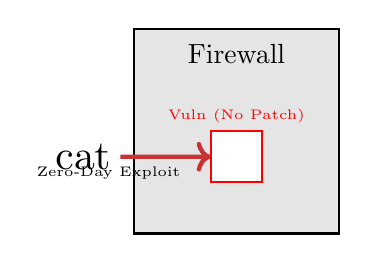
\begin{tikzpicture}[scale=0.65]
                    \fill[gray!20] (0,0) rectangle (4,4);
                    \draw[thick] (0,0) rectangle (4,4);
                    \node at (2, 3.5) {Firewall};
                    \fill[white] (1.5, 1) rectangle (2.5, 2);
                    \draw[red, thick] (1.5, 1) rectangle (2.5, 2);
                    \node[font=\tiny, text=red] at (2, 2.3) {Vuln (No Patch)};
                    \node (cat) at (-1, 1.5) {\iconcat[0.7cm]};
                    \draw[->, ultra thick, alertred] (cat) -- (1.5, 1.5);
                    \node[font=\tiny, below] at (-0.5, 1.5) {Zero-Day Exploit};
                \end{tikzpicture}
            \end{center}
        \end{column}
    \end{columns}
\end{frame}

% SLIDE 7: Deception Technologies
\begin{frame}{Defense Tool: Honeypots and Deception}
    \begin{columns}[T]
        \begin{column}{0.48\textwidth}
            \begin{block}{What is a Honeypot?}
                \footnotesize
                A "Trap Server" designed to look juicy to hackers.
                \begin{itemize}
                    \item \textbf{Purpose}: To waste the attacker's time and study their methods.
                    \item If anyone touches the Honeypot, \textbf{it's an attack} (because no real users should be there).
                \end{itemize}
            \end{block}
            \begin{exampleblock}{Common Tools}
                \footnotesize
                \textbf{Canary}: A device that chirps (alerts) when accessed.\\
                \textbf{Cowrie}: A fake SSH terminal that logs the hacker's commands.
            \end{exampleblock}
        \end{column}
        \begin{column}{0.48\textwidth}
            \begin{center}
                \begin{tikzpicture}[scale=0.7]
                    \node[draw, fill=green!10, rounded corners] (real) at (0, 3) {\icondatabase[0.8cm]};
                    \node[right, font=\tiny] at (0.5, 3) {Real DB};
                    \node[draw, fill=orange!20, rounded corners] (honey) at (0, 0) {\faIcon{archive}};
                    \node[right, font=\tiny] at (0.5, 0) {Honeypot};
                    \node[font=\tiny, text=orange] at (0, -0.8) {(Fake Data)};
                    \node (cat) at (-3, 1.5) {\iconcat[0.8cm]};
                    \draw[->, thick, green!50!black, dashed] (cat) -- (real) node[midway, sloped, above, font=\tiny] {Ignored};
                    \draw[->, ultra thick, red] (cat) -- (honey) node[midway, sloped, below, font=\tiny] {Attacks Here};
                    \node (snoopy) at (2.5, 0) {\icondog[0.6cm]};
                    \draw[->, thick, blue] (honey) -- (snoopy) node[midway, above, font=\tiny] {Alert!};
                \end{tikzpicture}
            \end{center}
        \end{column}
    \end{columns}
\end{frame}

% SLIDE 8: Threat Assessment (Detail Enhanced)
\begin{frame}{9.2 Threat Types and Assessment}
    \begin{columns}[T]
        \begin{column}{0.48\textwidth}
            \begin{block}{The Attacker Hierarchy}
                \footnotesize
                \begin{itemize}
                    \item \textbf{Script Kiddies}: Unskilled amateurs using tools they downloaded (Low threat).
                    \item \textbf{APTs (Nation-States)}: Highly skilled, government-funded spies (High threat).
                \end{itemize}
            \end{block}
            \begin{alertblock}{The Insider Threat}
                \footnotesize
                Current or former employees.
                \begin{itemize}
                    \item \textbf{Malicious}: Angry ex-admin.
                    \item \textbf{Accidental}: Employee clicking a phishing link. (Most common!)
                \end{itemize}
            \end{alertblock}
        \end{column}
        \begin{column}{0.48\textwidth}
            \begin{center}
                \begin{tikzpicture}[scale=0.7]
                    \node[draw, dashed, gray, rounded corners, minimum width=3.5cm, minimum height=3cm] (office) at (0,0) {};
                    \node[above, gray] at (0, 1.6) {Internal Network};
                    \node (user) at (-0.8, 0) {\iconuser[0.6cm]};
                    \node[below, font=\tiny] at (-0.8, -0.4) {Insider (Trusted)};
                    \node (srv) at (0.8, 0.5) {\iconserver[0.6cm]};
                    \node (hacker) at (3, 2) {\iconcat[0.7cm]};
                    \node[right, font=\tiny, text=alertred] at (3.3, 2) {External (Blocked)};
                    \draw[->, thick, alertred] (hacker) -- (srv) node[midway, sloped, above, font=\tiny] {Firewall Blocks};
                    \draw[->, thick, orange] (user) -- (srv) node[midway, below, font=\tiny] {Direct Access};
                \end{tikzpicture}
            \end{center}
        \end{column}
    \end{columns}
\end{frame}

% SLIDE 9: DoS vs DDoS (Analogy Enhanced)
\begin{frame}{Denial of Service (DoS) vs. Distributed DoS (DDoS)}
    \begin{columns}[T]
        \begin{column}{0.48\textwidth}
            \begin{block}{The "Traffic Jam" Analogy}
                \footnotesize
                \begin{itemize}
                    \item \textbf{DoS}: One car parks in front of the store entrance. (Annoying, but easy to tow/block).
                    \item \textbf{DDoS}: Every car in the city drives to the store at once. (Catastrophic, impossible to clear quickly).
                \end{itemize}
            \end{block}
            \begin{block}{Goal}
                \footnotesize
                To attack \textbf{Availability}. The server isn't hacked, it's just overwhelmed.
            \end{block}
        \end{column}
        \begin{column}{0.48\textwidth}
            \begin{center}
                \begin{tikzpicture}[scale=0.55]
                    \node (target) at (0, -2) {\iconserver[0.8cm]};
                    \node[below, font=\tiny] at (0, -2.5) {Victim};
                    \node (bot1) at (1, 1) {\iconpc[0.4cm]};
                    \node (bot2) at (2, 1) {\iconpc[0.4cm]};
                    \node (bot3) at (3, 1) {\iconpc[0.4cm]};
                    \node[font=\tiny, text=alertred] at (2, 1.5) {Botnet (Traffic Jam)};
                    \node (master) at (2, 3) {\iconcat[0.6cm]};
                    \draw[->, dashed, gray] (master) -- (bot1);
                    \draw[->, dashed, gray] (master) -- (bot2);
                    \draw[->, dashed, gray] (master) -- (bot3);
                    \draw[->, thick, red] (bot1) -- (target);
                    \draw[->, thick, red] (bot2) -- (target);
                    \draw[->, thick, red] (bot3) -- (target);
                \end{tikzpicture}
            \end{center}
        \end{column}
    \end{columns}
\end{frame}

% SLIDE 10: Botnets (Detail Enhanced)
\begin{frame}{Botnets: The Zombie Army}
    \begin{columns}[T]
        \begin{column}{0.55\textwidth}
            \begin{block}{Who are the Zombies?}
                \footnotesize
                Often insecure \textbf{IoT (Internet of Things)} devices:
                \begin{itemize}
                    \item Smart Cameras, Smart Bulbs, Connected Fridges.
                    \item Weak passwords make them easy targets!
                \end{itemize}
            \end{block}
            \begin{block}{Structure}
                \footnotesize
                \begin{enumerate}
                    \item \textbf{Herder}: The criminal.
                    \item \textbf{C\&C}: Server giving orders.
                    \item \textbf{Zombies}: The infected devices.
                \end{enumerate}
            \end{block}
        \end{column}
        \begin{column}{0.42\textwidth}
            \begin{center}
                \begin{tikzpicture}[scale=0.7]
                    \node (cc) at (0, 3) {\iconcloud[0.8cm]};
                    \node[right, font=\tiny] at (0.5, 3) {C\&C Server};
                    \node[opacity=0.5] (z1) at (-1.5, 1) {\faIcon{video}};
                    \node[opacity=0.5] (z2) at (0, 1) {\faIcon{video}};
                    \node[opacity=0.5] (z3) at (1.5, 1) {\faIcon{video}};
                    \node[font=\tiny] at (0, 0.5) {Hacked Cameras};
                    \fill[green] (-1.5, 1.1) circle (1pt);
                    \fill[green] (0, 1.1) circle (1pt);
                    \fill[green] (1.5, 1.1) circle (1pt);
                    \draw[->, dashed, red] (cc) -- (z1);
                    \draw[->, dashed, red] (cc) -- (z2);
                    \draw[->, dashed, red] (cc) -- (z3);
                \end{tikzpicture}
            \end{center}
        \end{column}
    \end{columns}
\end{frame}

% =============================================================================
% Module 9.0: Slides 11-21 (Enhanced Detail)
% =============================================================================

% SLIDE 11: Malware Zoo (Virus vs Worm)
\begin{frame}{Malware: Virus vs. Worm}
    \begin{columns}[T]
        \begin{column}{0.48\textwidth}
            \begin{block}{Virus (Needs a Driver)}
                \footnotesize
                Like a car that needs a driver, a Virus needs **YOU** to start it.
                \begin{itemize}
                    \item It hides inside a legitimate file (game, document, script).
                    \item It only infects when you \textbf{open/run} that file.
                \end{itemize}
            \end{block}
            \begin{block}{Worm (Self-Driving)}
                \footnotesize
                A Worm is a **self-driving car**.
                \begin{itemize}
                    \item It doesn't need a host file or a user.
                    \item It scans the network, finds a hole in a neighbor's computer, and jumps over automatically.
                    \item \textbf{Much faster} spreading than viruses.
                \end{itemize}
            \end{block}
        \end{column}
        \begin{column}{0.48\textwidth}
            \begin{center}
                \begin{tikzpicture}[scale=0.6]
                    % Virus
                    \node[draw, fill=gray!10] (file) at (0, 3) {\iconfile[0.8cm]};
                    \node[font=\tiny] at (0, 2.4) {InfectedFile.exe};
                    \node[text=alertred] at (0.3, 2.7) {\faIcon{bug}}; 
                    \node[right, font=\tiny, text=gray] at (1, 3) {Needs "Click"};

                    % Worm
                    \node (pc1) at (-2, 0) {\iconpc[0.6cm]};
                    \node (pc2) at (2, 0) {\iconpc[0.6cm]};
                    
                    % Snake decoration (Modern Syntax)
                    \draw[->, thick, red, decorate, decoration={snake, amplitude=.4mm, segment length=2mm, post length=1mm}] (pc1) -- (pc2) node[midway, above, font=\tiny] {Jumps Automatically!};
                    
                    \node[font=\tiny] at (0, -0.5) {Network Cable};
                \end{tikzpicture}
            \end{center}
        \end{column}
    \end{columns}
\end{frame}

% SLIDE 12: Malware Zoo (Trojan vs Ransomware)
\begin{frame}{Malware: Trojans \& Ransomware}
    \begin{columns}[T]
        \begin{column}{0.48\textwidth}
            \begin{block}{Trojan Horse (The Trick)}
                \footnotesize
                Named after the Greek myth. It looks like a gift, but contains soldiers (malware).
                \begin{itemize}
                    \item \textit{"Download this Screen Saver!"}
                    \item Screen saver runs, but it opens a \textbf{Backdoor} for the hacker.
                \end{itemize}
            \end{block}
            \begin{alertblock}{Ransomware (The Kidnapper)}
                \footnotesize
                It doesn't steal data; it \textbf{locks} it.
                \begin{itemize}
                    \item Encrypts your homework/photos.
                    \item Demands Crypto (Bitcoin) to buy the key.
                    \item \textit{Advice:} Never pay! (Restore from Backup).
                \end{itemize}
            \end{alertblock}
        \end{column}
        \begin{column}{0.48\textwidth}
            \begin{center}
                \begin{tikzpicture}[scale=0.7]
                    % Trojan
                    \node (gift) at (0, 2.5) {\faIcon{gift}};
                    \node[font=\tiny] at (0, 3) {FreeGame.exe};
                    \node (cat) at (0, 2.5) {\tiny \textcolor{alertred}{\faIcon{cat}}}; 
                    \node[right, font=\tiny, text=gray] at (0.5, 2.5) {Hidden Inside};
                    
                    % Ransomware
                    \node[draw, fill=red!10, minimum width=2cm, minimum height=1.5cm] (screen) at (0, 0) {};
                    \node[text=alertred] at (0, 0.2) {\iconlock[0.5cm]};
                    \node[font=\tiny, below] at (0, -0.2) {File Encrypted!};
                    \node[font=\tiny, below] at (0, -0.6) {Pay 5 BTC};
                \end{tikzpicture}
            \end{center}
        \end{column}
    \end{columns}
\end{frame}

% SLIDE 13: Case Study - The Zombie Accountants
\begin{frame}{Case Study: The Zombie Accountants}
    \begin{block}{Scenario: 2:00 AM Alert}
        \footnotesize
        Agent Snoopy's pager buzzes. The KibbleCorp webstore has crashed.
        
        He checks the network dashboard:
        \begin{itemize}
            \item The computers in the Accounting Department are all turned ON (they should be off).
            \item They are sending thousands of requests per second to the webstore.
            \item The accountants are asleep at home.
        \end{itemize}
    \end{block}
    \vspace{0.3cm}
    \begin{columns}[T]
        \begin{column}{0.7\textwidth}
            \textbf{Detective Questions:}
            \begin{enumerate}
                \item Why did the malware likely spread as a \textbf{Worm} instead of a Virus?
                \item The computers are acting as a group. What is this "Army" called?
                \item Is the attack trying to steal data or stop the business?
            \end{enumerate}
        \end{column}
        \begin{column}{0.25\textwidth}
            \begin{center}
                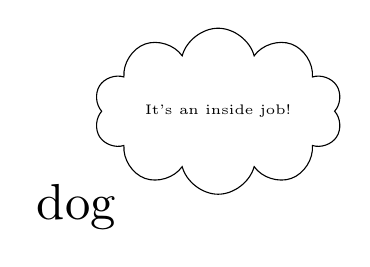
\begin{tikzpicture}
                    \node (snoopy) {\icondog[1cm]};
                    \node[above right=0.1cm of snoopy, cloud, draw, aspect=2, font=\tiny] {It's an inside job!};
                \end{tikzpicture}
            \end{center}
        \end{column}
    \end{columns}
\end{frame}

% SLIDE 14: Case Study Solution
\begin{frame}{Case Study Solution: The Zombie Accountants}
    \begin{exampleblock}{Snoopy's Analysis}
        \footnotesize
        \begin{enumerate}
            \item \textbf{Propagation:} It must be a \textbf{Worm} because it spread automatically while no one was using the computers.
            \item \textbf{The Army:} They are a \textbf{Botnet} (Robot Network) of Zombies.
            \item \textbf{Goal:} This is a \textbf{DDoS (Distributed Denial of Service)}. The goal is to overwhelm the webstore (Availability), not steal data (Confidentiality).
        \end{enumerate}
    \end{exampleblock}
    \begin{center}
        \begin{tikzpicture}[scale=0.6]
            \node (pc1) at (-4, 1) {\iconpc[0.5cm]};
            \node (pc2) at (-4, 0) {\iconpc[0.5cm]};
            \node (pc3) at (-4, -1) {\iconpc[0.5cm]};
            \node[below, font=\tiny] at (-4, -1.5) {Accounting (Zombies)};
            
            \node (target) at (2, 0) {\iconserver[0.6cm]};
            \node[right, font=\tiny] at (2.5, 0) {Webstore};
            
            \draw[->, ultra thick, alertred] (pc1) -- (target);
            \draw[->, ultra thick, alertred] (pc2) -- (target);
            \draw[->, ultra thick, alertred] (pc3) -- (target);
            
            \node (snoopy) at (0, -2) {\icondog[0.5cm]};
            \node[right, font=\tiny, text=rctcblue] at (0.3, -2) {Pull the network plug!};
        \end{tikzpicture}
    \end{center}
\end{frame}

% SLIDE 15: Spoofing Defined
\begin{frame}{9.3 Spoofing: The Fake Return Address}
    \begin{columns}[T]
        \begin{column}{0.48\textwidth}
            \begin{block}{What is Spoofing?}
                \footnotesize
                Falsifying data to gain an illegitimate advantage.
                \begin{itemize}
                    \item \textbf{IP Spoofing}: Writing a fake "Return Address" on a packet.
                    \item \textbf{Caller ID Spoofing}: Scammers calling from "Your Bank" (when they are really in a basement).
                \end{itemize}
            \end{block}
            \begin{alertblock}{Why does this work?}
                \footnotesize
                The Internet (IP) is like the Mail System. It delivers to the \textbf{Destination}. It rarely checks if the \textbf{Sender} is telling the truth!
            \end{alertblock}
        \end{column}
        \begin{column}{0.48\textwidth}
            \begin{center}
                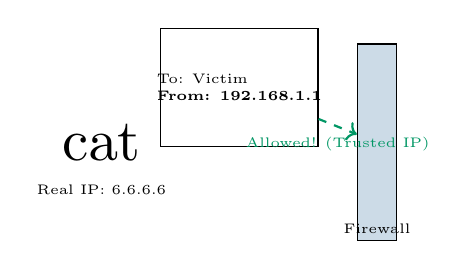
\begin{tikzpicture}[scale=0.7]
                    % Real Identity
                    \node (cat) at (0, 0) {\iconcat[1cm]};
                    \node[below, font=\tiny] at (0, -0.6) {Real IP: 6.6.6.6};
                    
                    % The Packet
                    \node[draw, fill=white, minimum width=2cm, minimum height=1.5cm] (pkt) at (2.5, 1) {};
                    \node[font=\tiny, align=left] at (2.5, 1) {To: Victim\\ \textbf{From: 192.168.1.1}};
                    
                    % Firewall
                    \node[draw, fill=rctcblue!20, minimum height=2.5cm, minimum width=0.5cm] (fw) at (5, 0) {};
                    \node[below, font=\tiny] at (5, -1.3) {Firewall};
                    
                    % Action
                    \draw[->, thick, dashed, networkgreen] (pkt) -- (fw) node[midway, below, font=\tiny] {Allowed! (Trusted IP)};
                \end{tikzpicture}
            \end{center}
        \end{column}
    \end{columns}
\end{frame}

% SLIDE 16: On-Path Attacks
\begin{frame}{On-Path Attacks (The "Middle Man")}
    \begin{columns}[T]
        \begin{column}{0.55\textwidth}
            \begin{block}{Concept: Passing Notes}
                \footnotesize
                Imagine Lucy passes a note to Linus in class.
                \begin{itemize}
                    \item The Hacker Cat sits between them.
                    \item He takes Lucy's note, reads it, \textbf{changes the words}, and passes it to Linus.
                    \item Linus thinks the note came from Lucy.
                \end{itemize}
                This is an **On-Path** (formerly Man-in-the-Middle) attack.
            \end{block}
            \begin{exampleblock}{Tools}
                \footnotesize
                \textbf{Wireshark} (to listen) and \textbf{Ettercap} (to intercept).
            \end{exampleblock}
        \end{column}
        \begin{column}{0.42\textwidth}
            \begin{center}
                \begin{tikzpicture}[scale=0.7]
                    \node (user) at (-2, 2) {\iconuser[0.5cm]};
                    \node (server) at (2, 2) {\iconserver[0.5cm]};
                    \draw[dashed, gray, opacity=0.5] (user) -- (server) node[midway, above, font=\tiny] {Normal Path};
                    
                    \node (attacker) at (0, 0) {\iconcat[0.8cm]};
                    \node[below, font=\tiny, text=alertred] at (0, -0.5) {On-Path Attacker};
                    
                    \draw[->, thick, alertred] (user) -- (attacker);
                    \draw[->, thick, alertred] (attacker) -- (server);
                    
                    \node[font=\tiny, fill=white] at (-1, 1) {Hello};
                    \node[font=\tiny, fill=white] at (1, 1) {Goodbye};
                \end{tikzpicture}
            \end{center}
        \end{column}
    \end{columns}
\end{frame}

% SLIDE 17: ARP Poisoning
\begin{frame}{ARP Poisoning: The Roll Call Lie}
    \begin{columns}[T]
        \begin{column}{0.48\textwidth}
            \begin{block}{The Vulnerability}
                \footnotesize
                ARP is the protocol that finds MAC addresses ("Who has IP 10.1.1.1?").
                \begin{itemize}
                    \item \textbf{Problem}: ARP has no ID check.
                    \item \textbf{Analogy}: The teacher calls "Linus?", and the Bully yells "Here!" The teacher marks the Bully as Linus.
                \end{itemize}
            \end{block}
            \begin{alertblock}{The Result}
                \footnotesize
                The Hacker Cat tells your computer "I am the Router." Your computer believes him and sends all your internet traffic to the Cat.
            \end{alertblock}
        \end{column}
        \begin{column}{0.48\textwidth}
            \begin{center}
                \begin{tikzpicture}[scale=0.65]
                    \node (vic) at (-2, 2) {\iconpc[0.6cm]};
                    \node[above, font=\tiny] at (-2, 2.3) {Victim};
                    
                    \node (rtr) at (2, 2) {\iconrouter[0.6cm]};
                    \node[above, font=\tiny] at (2, 2.3) {Router};
                    
                    \node (att) at (0, 0) {\iconcat[0.6cm]};
                    \node[below, font=\tiny] at (0, -0.5) {Hacker Cat};
                    
                    \node[draw, fill=white, font=\tiny, align=center] at (-2, 0.5) {ARP Table:\\Router = Cat};
                    
                    \draw[->, thick, alertred] (att) -- (vic) node[midway, left, font=\tiny] {"I am Router!"};
                    \draw[->, thick, alertred] (att) -- (rtr) node[midway, right, font=\tiny] {"I am Victim!"};
                \end{tikzpicture}
            \end{center}
        \end{column}
    \end{columns}
\end{frame}

% SLIDE 18: MAC Spoofing
\begin{frame}{Tool Spotlight: MAC Spoofing}
    \begin{columns}[T]
        \begin{column}{0.48\textwidth}
            \begin{block}{Changing Plates}
                \footnotesize
                Your MAC address is burned into the hardware, but software can override it.
                \begin{itemize}
                    \item \textbf{Analogy}: Putting fake license plates on a getaway car.
                    \item The camera (Switch/Router) sees the fake plate and lets the car through.
                \end{itemize}
            \end{block}
            \begin{block}{Why do it?}
                \footnotesize
                \begin{enumerate}
                    \item To bypass \textbf{MAC Filtering} (Access Control Lists).
                    \item To hide the device manufacturer (OUI) so hackers don't know what you are using.
                \end{enumerate}
            \end{block}
        \end{column}
        \begin{column}{0.48\textwidth}
            \begin{center}
                \begin{tikzpicture}[scale=0.6]
                    \node (pc) at (0, 0) {\iconpc[0.8cm]};
                    \node[below, font=\tiny] at (0, -0.5) {My Laptop};
                    
                    % Real MAC
                    \node[draw, dashed, gray, font=\tiny] at (0, 2) {Real: AA:BB:CC};
                    
                    % Fake MAC (Sticker)
                    \node[draw, fill=yellow!20, font=\tiny, rotate=10] at (0, 1.5) {Spoof: 11:22:33};
                    
                    \node (snoopy) at (3, 0) {\icondog[0.6cm]};
                    \node[right, font=\tiny, align=left] at (3.5, 0) {Looks like\\a new PC!};
                \end{tikzpicture}
            \end{center}
        \end{column}
    \end{columns}
\end{frame}

% SLIDE 19: VLAN Hopping
\begin{frame}{VLAN Hopping (Double Tagging)}
    \begin{columns}[T]
        \begin{column}{0.55\textwidth}
            \begin{block}{The Hidden Suitcase}
                \footnotesize
                How do you sneak a forbidden item past a checkpoint?
                \begin{itemize}
                    \item \textbf{Double Tagging}: Put a packet inside a packet.
                    \item \textbf{Outer Tag (VLAN 10)}: "This is for the lobby." The first switch opens it.
                    \item \textbf{Inner Tag (VLAN 20)}: "This is for the Secure Vault." The switch sees this \textit{after} opening the first one and sends it to the vault!
                \end{itemize}
            \end{block}
        \end{column}
        \begin{column}{0.42\textwidth}
            \begin{center}
                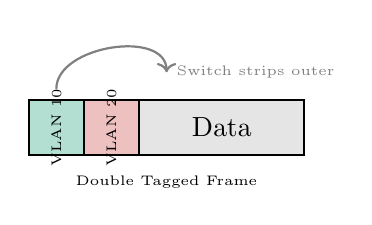
\begin{tikzpicture}[scale=0.7]
                    % Data
                    \draw[thick, fill=gray!20] (0, 0) rectangle (3, 1);
                    \node at (1.5, 0.5) {Data};
                    
                    % Inner Tag
                    \draw[thick, fill=alertred!30] (-1, 0) rectangle (0, 1);
                    \node[font=\tiny, rotate=90] at (-0.5, 0.5) {VLAN 20};
                    
                    % Outer Tag
                    \draw[thick, fill=networkgreen!30] (-2, 0) rectangle (-1, 1);
                    \node[font=\tiny, rotate=90] at (-1.5, 0.5) {VLAN 10};
                    
                    % Explanation
                    \node[below, font=\tiny] at (0.5, -0.2) {Double Tagged Frame};
                    \draw[->, thick, gray] (-1.5, 1.2) to [out=90,in=90] (0.5, 1.5) node[right, font=\tiny] {Switch strips outer};
                \end{tikzpicture}
            \end{center}
        \end{column}
    \end{columns}
\end{frame}

% SLIDE 20: Case Study - Snoopy at the Cafe
\begin{frame}{Case Study: The Coffee Shop Interception}
    \begin{block}{Scenario: Free Wi-Fi Danger}
        \footnotesize
        Agent Snoopy is at the "KibbleKafe." He connects to the open Wi-Fi to check his bank.
        
        The Hacker Cat is sitting in the corner. Suddenly, Snoopy's browser warns:
        
        \textbf{"Certificate Error: The identity of bank.com cannot be verified."}
        
        Snoopy realizes his traffic is being detoured through the Cat's laptop.
    \end{block}
    \vspace{0.3cm}
    \begin{columns}[T]
        \begin{column}{0.7\textwidth}
            \textbf{Detective Questions:}
            \begin{enumerate}
                \item What Layer 2 protocol is the Hacker Cat abusing to redirect the traffic?
                \item What is the Hacker Cat's position called (sitting between Snoopy and the Router)?
                \item Why did Snoopy see a Certificate Error (HTTPS)?
            \end{enumerate}
        \end{column}
        \begin{column}{0.25\textwidth}
            \begin{center}
                \begin{tikzpicture}
                    \node (cat) {\iconcat[1cm]};
                    \node[above, font=\tiny] at (0, 0.6) {Evil Grin};
                    \node (wifi) at (1, 1) {\faIcon{wifi}};
                \end{tikzpicture}
            \end{center}
        \end{column}
    \end{columns}
\end{frame}

% SLIDE 21: Case Study Solution
\begin{frame}{Case Study Solution: The Coffee Shop Interception}
    \begin{exampleblock}{Analysis}
        \footnotesize
        \begin{enumerate}
            \item \textbf{Protocol:} \textbf{ARP}. The Cat used ARP Poisoning to tell Snoopy "I am the Router."
            \item \textbf{Position:} \textbf{On-Path (Man-in-the-Middle)}.
            \item \textbf{Error:} The Cat tried to read encrypted (HTTPS) traffic. Since he doesn't have the Bank's private key, he used a fake certificate. Snoopy's browser detected the fake.
        \end{enumerate}
    \end{exampleblock}
    \begin{center}
        \begin{tikzpicture}[scale=0.6]
            \node (snoopy) at (-3, 0) {\icondog[0.6cm]};
            \node (cat) at (0, 0) {\iconcat[0.8cm]};
            \node (router) at (3, 0) {\iconrouter[0.6cm]};
            
            \draw[->, thick, alertred, bend left] (snoopy) to node[above, font=\tiny] {Traffic} (cat);
            \draw[->, thick, alertred, bend left] (cat) to node[above, font=\tiny] {Traffic} (router);
            
            \node[below, font=\tiny] at (0, -0.8) {The "Middle Man"};
        \end{tikzpicture}
    \end{center}
\end{frame}

% =============================================================================
% Module 9.0: Slides 22-40 (Rogue Systems, Social Eng, Review)
% =============================================================================

% SLIDE 22: Rogue Devices
\begin{frame}{9.4 Rogue Devices and Evil Twins}
    \begin{columns}[T]
        \begin{column}{0.48\textwidth}
            \begin{block}{Rogue Devices}
                \footnotesize
                Unauthorized hardware plugged into the network.
                \begin{itemize}
                    \item Employee brings a home router to get better Wi-Fi.
                    \item Hacker hides a "Raspberry Pi" behind a printer.
                \end{itemize}
            \end{block}
            \begin{alertblock}{The Evil Twin (Wi-Fi)}
                \footnotesize
                \textbf{The "Fake Starbucks" Attack.}
                \begin{itemize}
                    \item Attacker sets up a Wi-Fi spot with the \textbf{exact same name} (SSID) as the real one.
                    \item Your phone sees two "KibbleCorp-WiFi" networks.
                    \item It connects to the \textbf{strongest signal} (the attacker), giving them your data.
                \end{itemize}
            \end{alertblock}
        \end{column}
        \begin{column}{0.48\textwidth}
            \begin{center}
                \begin{tikzpicture}[scale=0.7]
                    % Real AP
                    \node (real) at (-2, 2) {\faIcon{wifi}};
                    \node[above, font=\tiny, text=networkgreen] at (-2, 2.3) {Corp-WiFi (Real)};
                    
                    % Evil Twin
                    \node (fake) at (2, 2) {\faIcon{wifi}};
                    \node[above, font=\tiny, text=alertred] at (2, 2.3) {Corp-WiFi (Fake)};
                    \node at (2, 1.5) {\iconcat[0.5cm]};
                    
                    % Victim
                    \node (vic) at (0, 0) {\iconpc[0.6cm]};
                    
                    % Signal strength
                    \draw[->, dashed, thick, alertred] (fake) -- (vic) node[midway, right, font=\tiny] {Stronger Signal!};
                    \draw[->, dashed, gray] (real) -- (vic) node[midway, left, font=\tiny] {Weaker};
                \end{tikzpicture}
            \end{center}
        \end{column}
    \end{columns}
\end{frame}

% SLIDE 23: Rogue DHCP
\begin{frame}{Rogue DHCP Servers}
    \begin{columns}[T]
        \begin{column}{0.48\textwidth}
            \begin{block}{The Danger}
                \footnotesize
                If an attacker plugs in a router, it might start handing out IP addresses.
            \end{block}
            \begin{alertblock}{The "Race" Condition}
                \footnotesize
                Clients accept the \textbf{first} DHCP OFFER they receive.
                \begin{itemize}
                    \item \textbf{Real DHCP}: "Here is IP 10.1.1.5, Gateway is Router."
                    \item \textbf{Rogue DHCP}: "Here is IP 10.1.1.5, Gateway is \textbf{ME (The Cat)}."
                    \item Result: All internet traffic detours through the attacker.
                \end{itemize}
            \end{alertblock}
        \end{column}
        \begin{column}{0.48\textwidth}
            \begin{center}
                \begin{tikzpicture}[scale=0.6]
                    \node (client) at (0, 0) {\iconpc[0.6cm]};
                    \node[below, font=\tiny] at (0, -0.5) {Client Broadcasts DISCOVER};
                    
                    \node (real) at (-3, 3) {\iconserver[0.6cm]};
                    \node[above, font=\tiny] at (-3, 3.4) {Real DHCP};
                    
                    \node (rogue) at (3, 3) {\iconcat[0.6cm]};
                    \node[above, font=\tiny, text=alertred] at (3, 3.4) {Rogue DHCP};
                    
                    \draw[->, thick, green!50!black, dashed] (real) -- (client) node[midway, left, font=\tiny] {OFFER (Slow)};
                    \draw[->, thick, alertred] (rogue) -- (client) node[midway, right, font=\tiny] {OFFER (Fast!)};
                    
                    \node[draw, fill=white, font=\tiny] at (0, 1.5) {Winner sets the Gateway!};
                \end{tikzpicture}
            \end{center}
        \end{column}
    \end{columns}
\end{frame}

% SLIDE 24: DHCP Snooping (Defense)
\begin{frame}{Defending with DHCP Snooping}
    \begin{columns}[T]
        \begin{column}{0.48\textwidth}
            \begin{block}{The Solution: DHCP Snooping}
                \footnotesize
                A security feature on switches that acts like a \textbf{Club Bouncer}.
            \end{block}
            \begin{exampleblock}{Trust Boundaries}
                \footnotesize
                \begin{itemize}
                    \item \textbf{Trusted Ports}: Uplinks to real servers. \textit{"VIPs allowed to speak."}
                    \item \textbf{Untrusted Ports}: Regular user ports. \textit{"You can listen, but you cannot hand out IPs."}
                \end{itemize}
                If an OFFER packet comes from an Untrusted port, the switch \textbf{drops it}.
            \end{exampleblock}
        \end{column}
        \begin{column}{0.48\textwidth}
            \begin{center}
                \begin{tikzpicture}[scale=0.6]
                    % Switch
                    \node[draw, fill=rctcblue!10, minimum width=4cm, minimum height=1.5cm] (sw) at (0, 2) {};
                    \node at (0, 2) {\iconswitch[0.8cm]};
                    
                    % Trusted
                    \node (uplink) at (0, 4) {\iconserver[0.5cm]};
                    \draw[thick, green!50!black] (uplink) -- (0, 2.75);
                    \node[font=\tiny, fill=white, text=green!50!black] at (0, 3.2) {Trusted Port};
                    
                    % Untrusted User
                    \node (user) at (-2, 0) {\iconpc[0.5cm]};
                    \draw[thick, green!50!black] (user) -- (-1.5, 1.25);
                    
                    % Untrusted Attacker
                    \node (cat) at (2, 0) {\iconcat[0.5cm]};
                    \draw[thick, red] (cat) -- (1.5, 1.25);
                    
                    % Drop Logic
                    \node[draw, circle, fill=alertred, text=white, font=\bfseries\tiny] at (1.5, 1.25) {X};
                    \node[font=\tiny, text=alertred] at (2.5, 1) {OFFER Dropped!};
                \end{tikzpicture}
            \end{center}
        \end{column}
    \end{columns}
\end{frame}

% SLIDE 25: DNS Attacks
\begin{frame}{DNS Attacks: Poisoning the Phonebook}
    \begin{columns}[T]
        \begin{column}{0.48\textwidth}
            \begin{block}{Concept: The Phonebook}
                \footnotesize
                DNS turns Names (google.com) into Numbers (8.8.8.8).
            \end{block}
            \begin{alertblock}{DNS Poisoning}
                \footnotesize
                \textbf{"Changing the entry in the book."}
                \begin{itemize}
                    \item Attacker hacks the DNS Server.
                    \item Changes "BankOfAmerica.com" to the Attacker's IP.
                    \item You type the correct URL, but your browser goes to the \textbf{fake site}.
                \end{itemize}
            \end{alertblock}
        \end{column}
        \begin{column}{0.48\textwidth}
            \begin{center}
                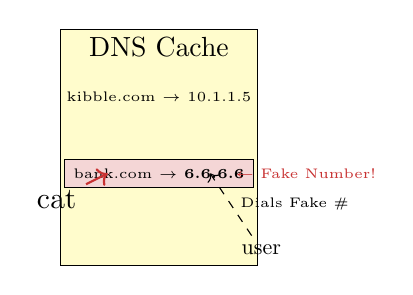
\begin{tikzpicture}[scale=0.65]
                    \node[draw, fill=yellow!20, minimum width=2.5cm, minimum height=3cm] (book) at (0,0) {};
                    \node[above] at (0, 1.6) {DNS Cache};
                    
                    \node[font=\tiny] at (0, 1) {kibble.com $\to$ 10.1.1.5};
                    \node[draw, fill=alertred!20, font=\tiny] at (0, -0.5) {bank.com $\to$ \textbf{6.6.6.6}};
                    \node[right, font=\tiny, text=alertred] at (1.3, -0.5) {$\leftarrow$ Fake Number!};
                    
                    \node (cat) at (-2, -1) {\iconcat[0.5cm]};
                    \draw[->, thick, alertred] (cat) -- (-1, -0.5);
                    
                    \node (user) at (2, -2) {\iconuser[0.5cm]};
                    \draw[->, dashed] (user) -- (1, -0.5) node[midway, right, font=\tiny] {Dials Fake \#};
                \end{tikzpicture}
            \end{center}
        \end{column}
    \end{columns}
\end{frame}

% SLIDE 26: Social Engineering
\begin{frame}{9.5 Social Engineering: Hacking the Human}
    \begin{columns}[T]
        \begin{column}{0.48\textwidth}
            \begin{block}{Phishing (The Bait)}
                \footnotesize
                Sending fraudulent messages to trick users.
                \begin{itemize}
                    \item \textbf{Phishing}: Regular email scams ("You won a prize!").
                    \item \textbf{Spear Phishing}: Targeted ("Hi Linus, this is your boss...").
                    \item \textbf{Whaling}: Targeting the CEO/Big Fish.
                \end{itemize}
            \end{block}
            \begin{block}{Other Variants}
                \footnotesize
                \begin{itemize}
                    \item \textbf{Vishing}: Voice/Phone (Scam calls).
                    \item \textbf{Smishing}: SMS/Text messages.
                \end{itemize}
            \end{block}
        \end{column}
        \begin{column}{0.48\textwidth}
            \begin{center}
                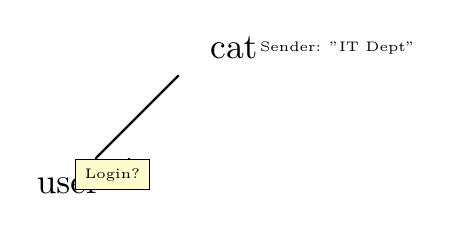
\begin{tikzpicture}[scale=0.7]
                    \node (user) at (0, 0) {\iconuser[0.8cm]};
                    \draw[thick] (2, 2) -- (0.5, 0.5);
                    \draw[thick] (0.5, 0.5) arc (180:360:0.3);
                    \node[font=\tiny, draw, fill=yellow!20] at (0.8, 0.2) {Login?};
                    \node (cat) at (3, 2.5) {\iconcat[0.6cm]};
                    \node[right, font=\tiny] at (3.3, 2.5) {Sender: "IT Dept"};
                \end{tikzpicture}
            \end{center}
        \end{column}
    \end{columns}
\end{frame}

% SLIDE 27: Physical Social Eng
\begin{frame}{Physical Social Engineering}
    \begin{columns}[T]
        \begin{column}{0.55\textwidth}
            \begin{block}{Techniques}
                \footnotesize
                \begin{itemize}
                    \item \textbf{Tailgating}: Following an authorized person through a secure door ("Hold the door, please!").
                    \item \textbf{Dumpster Diving}: Searching trash for sticky notes with passwords.
                    \item \textbf{Shoulder Surfing}: Watching someone type their PIN or password.
                \end{itemize}
            \end{block}
        \end{column}
        \begin{column}{0.42\textwidth}
            \begin{center}
                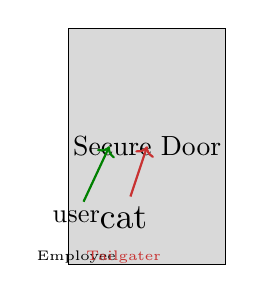
\begin{tikzpicture}[scale=0.6]
                    \node[draw, fill=gray!30, minimum width=2cm, minimum height=3cm] (door) at (0, 2) {};
                    \node at (0, 2) {Secure Door};
                    
                    \node (emp) at (-1.5, 0.5) {\iconuser[0.6cm]};
                    \node[below, font=\tiny] at (-1.5, 0) {Employee};
                    
                    \node (cat) at (-0.5, 0.5) {\iconcat[0.6cm]};
                    \node[below, font=\tiny, text=alertred] at (-0.5, 0) {Tailgater};
                    
                    \draw[->, thick, green!50!black] (emp) -- (-0.8, 2);
                    \draw[->, thick, alertred] (cat) -- (0, 2);
                \end{tikzpicture}
            \end{center}
        \end{column}
    \end{columns}
\end{frame}

% SLIDE 28: Principles of Influence
\begin{frame}{Principles of Influence}
    \begin{block}{Why does it work?}
        \footnotesize
        Attackers exploit human psychology ("Hacking the Human").
    \end{block}
    \vspace{0.2cm}
    \begin{columns}[T]
        \begin{column}{0.48\textwidth}
            \begin{itemize}
                \item \textbf{Authority}: "I am the CEO/Police, do this now!"
                \item \textbf{Intimidation}: "Do it or you're fired."
                \item \textbf{Consensus}: "Everyone else is doing it."
            \end{itemize}
        \end{column}
        \begin{column}{0.48\textwidth}
            \begin{itemize}
                \item \textbf{Scarcity}: "Only 2 iPhones left!"
                \item \textbf{Urgency}: "Account expires in 10 minutes!"
                \item \textbf{Trust}: "I know your friend Linus."
            \end{itemize}
        \end{column}
    \end{columns}
    \vspace{0.5cm}
    \begin{center}
        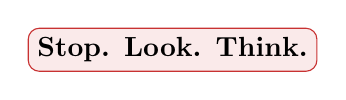
\begin{tikzpicture}
            \node[draw=alertred, fill=alertred!10, rounded corners, font=\bfseries] {Stop. Look. Think.};
        \end{tikzpicture}
    \end{center}
\end{frame}

% SLIDE 29: Password Attacks
\begin{frame}{Password Attacks}
    \begin{columns}[T]
        \begin{column}{0.48\textwidth}
            \begin{block}{Brute Force}
                \footnotesize
                Trying \textbf{every possible combination} (aaaa, aaab...).
                \begin{itemize}
                    \item \textit{Analogy:} Trying every single key on a keychain until one fits.
                    \item Guaranteed to work, but takes forever.
                \end{itemize}
            \end{block}
            \begin{block}{Dictionary Attack}
                \footnotesize
                Using a list of common words (dictionary).
                \begin{itemize}
                    \item \textit{Analogy:} Trying the most common house keys first.
                    \item Fails if the password is complex ("Xy9\#m!").
                \end{itemize}
            \end{block}
        \end{column}
        \begin{column}{0.48\textwidth}
            \begin{center}
                \begin{tikzpicture}[scale=0.7]
                    \node (lock) at (0, 2) {\iconlock[0.8cm]};
                    
                    \node[font=\tiny, align=left] at (-2, 0) {a...\\b...\\c...};
                    \draw[->, red] (-2, 0.5) -- (lock) node[midway, left, font=\tiny] {Slow};
                    
                    \node[draw, fill=white] (dict) at (2, 0) {\faIcon{book}};
                    \node[below, font=\tiny] at (2, -0.3) {Wordlist};
                    \draw[->, red] (dict) -- (lock) node[midway, right, font=\tiny] {Fast};
                \end{tikzpicture}
            \end{center}
        \end{column}
    \end{columns}
\end{frame}

% SLIDE 30: Password Tools & Salting
\begin{frame}{Tool Spotlight: John the Ripper \& Salting}
    \begin{columns}[T]
        \begin{column}{0.55\textwidth}
            \begin{block}{John the Ripper (JtR)}
                \footnotesize
                A tool used to test password strength by trying to crack them.
            \end{block}
            \begin{alertblock}{Defense: Salting}
                \footnotesize
                \textbf{"Adding Spice to the Recipe."}
                \begin{itemize}
                    \item Before saving a password, we add random characters ("Salt").
                    \item If Linus and Lucy both use "password123", their hashes will look completely different because they have different salts.
                    \item Prevents pre-calculated attacks (Rainbow Tables).
                \end{itemize}
            \end{alertblock}
        \end{column}
        \begin{column}{0.42\textwidth}
            \begin{center}
                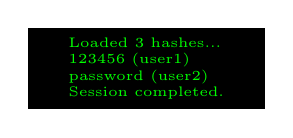
\begin{tikzpicture}[scale=0.6]
                    \node[draw, fill=black, text=green, font=\tiny, align=left, minimum width=3cm] {
                        Loaded 3 hashes...\\
                        123456 (user1)\\
                        password (user2)\\
                        Session completed.
                    };
                \end{tikzpicture}
            \end{center}
        \end{column}
    \end{columns}
\end{frame}

% SLIDE 31: Case Study - Intern Ike
\begin{frame}{Case Study: Intern Ike and the "CEO"}
    \begin{block}{Scenario: 4:55 PM on a Friday}
        \footnotesize
        Intern Ike at KibbleCorp receives an email:
        
        \vspace{0.2em}
        \textit{"From: ceo@kibble-corp.net (Notice the .net!)\\
        Subject: URGENT WIRE TRANSFER\\
        I am stuck in a meeting. Wire \$5,000 to this vendor immediately. If this isn't done by 5:00 PM, it will be your fault. Do it now!"}
    \end{block}
    \vspace{0.3cm}
    \begin{columns}[T]
        \begin{column}{0.7\textwidth}
            \textbf{Questions:}
            \begin{enumerate}
                \item What specific type of social engineering is this?
                \item Which "Principles of Influence" are being used?
                \item What should Ike do?
            \end{enumerate}
        \end{column}
        \begin{column}{0.25\textwidth}
            \begin{center}
                \begin{tikzpicture}
                    \node[draw, fill=yellow!10] {\faIcon{envelope-open-text}};
                    \node[font=\bfseries\huge, text=red] at (0.5, 0.5) {!};
                \end{tikzpicture}
            \end{center}
        \end{column}
    \end{columns}
\end{frame}

% SLIDE 32: Case Study Solution
\begin{frame}{Case Study Solution: Intern Ike}
    \begin{exampleblock}{Snoopy's Advice}
        \footnotesize
        \begin{enumerate}
            \item \textbf{Type:} \textbf{Whaling} (impersonating a big fish/exec) or Spear Phishing.
            \item \textbf{Principles:} 
            \begin{itemize}
                \item \textbf{Authority} ("I am the CEO").
                \item \textbf{Urgency} ("By 5:00 PM").
                \item \textbf{Intimidation} ("It will be your fault").
            \end{itemize}
            \item \textbf{Action:} \textbf{Verify Out-of-Band}. Do not reply to the email. Call the CEO's assistant or walk to their office. Report to Snoopy immediately.
        \end{enumerate}
    \end{exampleblock}
\end{frame}

% SLIDE 33: Recap
\begin{frame}{Recap: Offensive vs. Defensive}
    \begin{columns}[T]
        \begin{column}{0.48\textwidth}
            \begin{block}{The Attacker (Red Team)}
                \footnotesize
                \begin{itemize}
                    \item \textbf{Spoofing}: Hiding identity (Masks).
                    \item \textbf{Poisoning}: Redirecting traffic (Fake Signs).
                    \item \textbf{Cracking}: Breaking passwords (Lockpicking).
                \end{itemize}
            \end{block}
        \end{column}
        \begin{column}{0.48\textwidth}
            \begin{block}{The Defender (Blue Team)}
                \footnotesize
                \begin{itemize}
                    \item \textbf{Snooping}: Stopping rogue DHCP (Bouncers).
                    \item \textbf{Honeypots}: Trapping intruders (Decoys).
                    \item \textbf{Analysis}: Seeing the truth (Surveillance).
                \end{itemize}
            \end{block}
        \end{column}
    \end{columns}
    \vspace{0.5cm}
    \begin{center}
        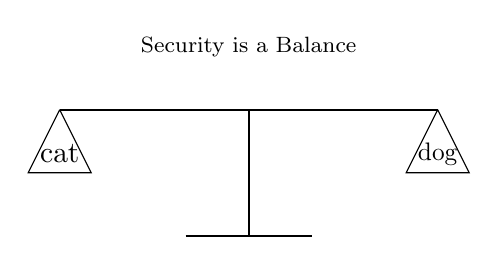
\begin{tikzpicture}[scale=0.8]
            \draw[thick] (0, 0) -- (6, 0); 
            \draw[thick] (3, 0) -- (3, -2); 
            \draw[thick] (2, -2) -- (4, -2); 
            
            \draw (0, 0) -- (-0.5, -1) -- (0.5, -1) -- (0, 0);
            \node at (0, -0.7) {\iconcat[0.5cm]};
            
            \draw (6, 0) -- (5.5, -1) -- (6.5, -1) -- (6, 0);
            \node at (6, -0.7) {\icondog[0.5cm]};
            
            \node[font=\footnotesize, align=center] at (3, 1) {Security is a Balance};
        \end{tikzpicture}
    \end{center}
\end{frame}

% SLIDE 34: Wireshark Analysis
\begin{frame}{Analyzing the Attack with Wireshark}
    \begin{columns}[T]
        \begin{column}{0.35\textwidth}
            \begin{block}{Red Flags}
                \footnotesize
                \begin{itemize}
                    \item \textbf{Flag 1}: Thousands of packets from one IP (DoS).
                    \item \textbf{Flag 2}: Duplicate IP addresses (ARP Poisoning).
                    \item \textbf{Flag 3}: Plaintext passwords (HTTP/Telnet).
                \end{itemize}
            \end{block}
        \end{column}
        \begin{column}{0.6\textwidth}
            \begin{center}
                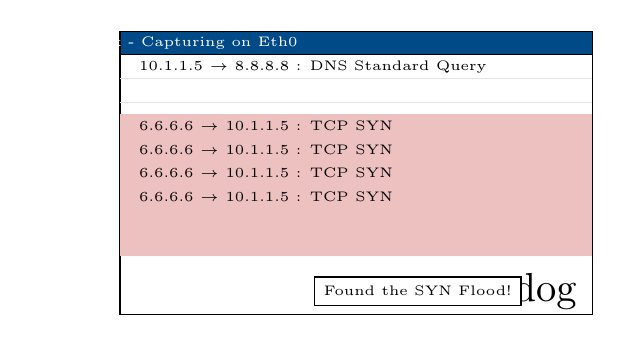
\begin{tikzpicture}[scale=0.6]
                    \draw[fill=white] (0, 0) rectangle (10, 6);
                    \draw[fill=rctcblue] (0, 5.5) rectangle (10, 6);
                    \node[white, font=\tiny] at (1, 5.75) {Wireshark - Capturing on Eth0};
                    
                    \foreach \y in {5, 4.5, 4, 3.5, 3, 2.5, 2, 1.5}
                        \draw[gray!20] (0, \y) -- (10, \y);
                        
                    \node[font=\tiny, anchor=west] at (0.2, 5.25) {10.1.1.5 $\to$ 8.8.8.8 : DNS Standard Query};
                    
                    % Attack Block
                    \fill[alertred!30] (0, 4.25) rectangle (10, 1.25);
                    \node[font=\tiny, anchor=west] at (0.2, 4.0) {6.6.6.6 $\to$ 10.1.1.5 : TCP SYN};
                    \node[font=\tiny, anchor=west] at (0.2, 3.5) {6.6.6.6 $\to$ 10.1.1.5 : TCP SYN};
                    \node[font=\tiny, anchor=west] at (0.2, 3.0) {6.6.6.6 $\to$ 10.1.1.5 : TCP SYN};
                    \node[font=\tiny, anchor=west] at (0.2, 2.5) {6.6.6.6 $\to$ 10.1.1.5 : TCP SYN};
                    
                    \node (snoopy) at (9, 0.5) {\icondog[0.8cm]};
                    \node[left, font=\tiny, fill=white, draw] at (8.5, 0.5) {Found the SYN Flood!};
                \end{tikzpicture}
            \end{center}
        \end{column}
    \end{columns}
\end{frame}

% SLIDE 35: Mitigation Strategies
\begin{frame}{Defense in Depth: Mitigation Strategies}
    \begin{center}
        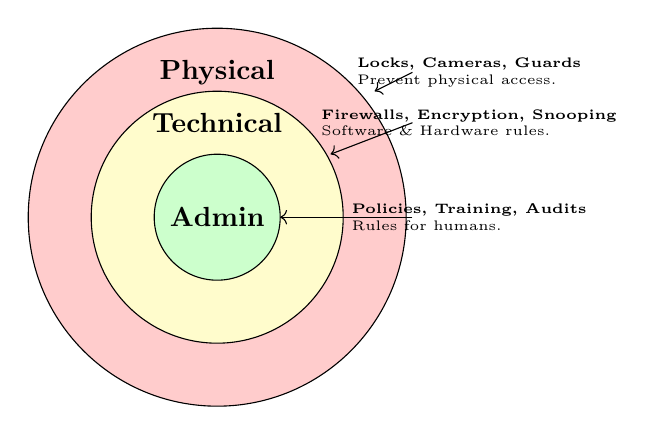
\begin{tikzpicture}[scale=0.8]
            \draw[fill=red!20] (0,0) circle (3cm);
            \node[font=\bfseries] at (0, 2.3) {Physical};
            
            \draw[fill=yellow!20] (0,0) circle (2cm);
            \node[font=\bfseries] at (0, 1.5) {Technical};
            
            \draw[fill=green!20] (0,0) circle (1cm);
            \node[font=\bfseries] at (0, 0) {Admin};
            
            \node[align=left, font=\tiny] at (4, 2.3) {\textbf{Locks, Cameras, Guards}\\Prevent physical access.};
            \draw[->] (3.1, 2.3) -- (2.5, 2);
            
            % Escaped Ampersand here
            \node[align=left, font=\tiny] at (4, 1.5) {\textbf{Firewalls, Encryption, Snooping}\\Software \& Hardware rules.};
            \draw[->] (3.1, 1.5) -- (1.8, 1);
            
            \node[align=left, font=\tiny] at (4, 0) {\textbf{Policies, Training, Audits}\\Rules for humans.};
            \draw[->] (3.1, 0) -- (1, 0);
        \end{tikzpicture}
    \end{center}
    \begin{alertblock}{No Single Solution}
        \footnotesize
        A firewall won't stop a user from holding the door open for a hacker. You need \textbf{all three layers} (Defense in Depth).
    \end{alertblock}
\end{frame}

% SLIDE 36: Resources
\begin{frame}{9.6 Additional Resources}
    \begin{columns}[T]
        \begin{column}{0.48\textwidth}
            \begin{block}{Vulnerability Databases}
                \footnotesize
                \begin{itemize}
                    \item \textbf{CVE (MITRE)}: The dictionary of vulnerabilities.
                    \item \textbf{NVD (NIST)}: Adds severity scores to CVEs.
                \end{itemize}
            \end{block}
            \begin{block}{Learning Tools}
                \footnotesize
                \begin{itemize}
                    \item \textbf{OWASP Top 10}: Web risks.
                    \item \textbf{TryHackMe}: Legal practice labs.
                \end{itemize}
            \end{block}
        \end{column}
        \begin{column}{0.48\textwidth}
            \begin{center}
                \begin{tikzpicture}
                    \node[draw, fill=white, drop shadow] (book) at (0,0) {\faIcon{book}};
                    \node[below] at (0, -0.5) {Knowledge is Power};
                    
                    \node (snoopy) at (2, 0) {\icondog[0.8cm]};
                    \node[right, font=\tiny, align=left] at (2.5, 0) {Read the docs\\before the\\hackers do!};
                \end{tikzpicture}
            \end{center}
        \end{column}
    \end{columns}
\end{frame}

% SLIDE 37: Questions
\begin{frame}{Questions?}
    \begin{center}
        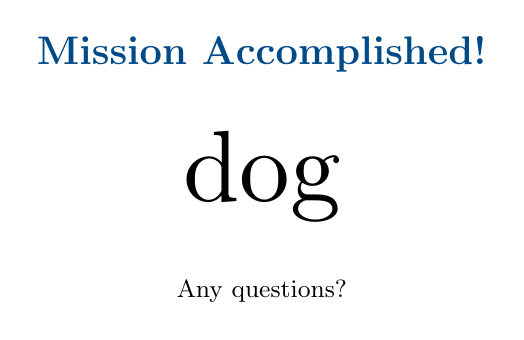
\begin{tikzpicture}[scale=1.5]
            \node (snoopy) at (0, 0) {\icondog[2cm]};
            \node[above=0.5cm of snoopy, font=\Large\bfseries, text=rctcblue] {Mission Accomplished!};
            \node[below=0.5cm of snoopy, font=\small] {Any questions?};
        \end{tikzpicture}
    \end{center}
\end{frame}



\end{document}